\documentclass{article}
\usepackage{alexconfig}
\usepackage{tikz}
\usetikzlibrary{calc}
\title{Carrol Chapter 2: Celestial Mechanics}

\begin{document}
\maketitle

\begin{definition}[Astronomical Units]
\

An \textbf{astronomical unit} (AU) is the average distance between the Earth and the Sun 
\end{definition}

\begin{proposition}[Kepler's Three Laws]
\

\begin{enumerate}
    \item A planet orbits the Sun in an ellipse, with the Sun at one focus of the ellipse
    \item A line connecting a planet to the Sun sweeps out equal areas in equal time intervals
    \item If $P$ is the sidereal period of a planet, and $a$ is the average distance of the planet from the Sun (in astronomical units), then they are related by $$P^2 = a^3$$
\end{enumerate}
\end{proposition}

\begin{definition}[Ellipses]
\

An \textbf{ellipse} is defined by two points, called \textbf{foci}, and consists of all of the points that satisfy the following equation:  $$r_1 + r_2 = 2a$$where $r_1$ and $r_2$ are distances from a point to the two foci, and $a$ is the length of the \textbf{semimajor axis}, or half the length of the longest axis of the ellipse. Half of the shorter axis $b$ is called the \textbf{semiminor axis}. 
\end{definition}

\begin{definition}[Eccentricity]
\

Let $d$ be the distance between the foci of an ellipse, and $a$ be the semimajor axis. Then, the \textbf{eccentricity}, which measures how "stretched" an ellipse is is given by $$e = \frac{d}{2a}$$  
\end{definition}

\begin{definition}[Points on an Ellipse]
\

The \textbf{aphelion} is the point fartherst from the foci of the ellipse, where the major axis meets the ellipse.

The \textbf{perihelion} is the point closest to the foci, where the minor axis meets the ellipse. 
\end{definition}

\begin{theorem}
\

Let $a$ be the semimajor axis of an ellipse, $b$ be the semiminor axis, $e$ be the eccentricity. Then, $$b^2 = a^2(1-e^2)$$
\end{theorem}

\begin{customproof}
\

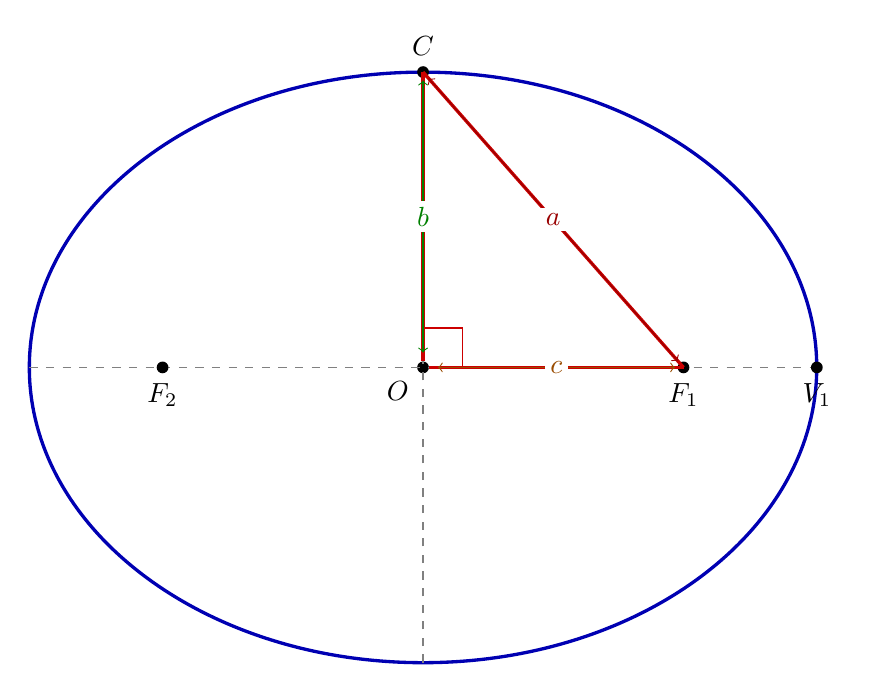
\begin{tikzpicture}[scale=2.5, dot/.style={fill, circle, inner sep=1.5pt}]

    % Define parameters (e.g., a=2, b=1.5, which gives c=1.32)
    \pgfmathsetmacro{\a}{2}  % Semi-major axis
    \pgfmathsetmacro{\b}{1.5} % Semi-minor axis
    \pgfmathsetmacro{\c}{sqrt(\a*\a - \b*\b)} % Distance from center to focus (c)

    % --- 1. Draw the Ellipse ---
    \draw[very thick, blue!70!black] (0,0) ellipse ({\a} and {\b});

    % --- 2. Mark the Center and Axes ---
    \node[dot, label={below left:$O$}] (O) at (0,0) {};
    
    % Draw the axes for reference (lighter lines)
    \draw[dashed, gray] (-\a,0) -- (\a,0);
    \draw[dashed, gray] (0,-\b) -- (0,\b);

    \coordinate (V1) at (\a, 0);     % Vertex 1 (A)
    \coordinate (V2) at (-\a, 0);    % Vertex 2 (-A)
    \coordinate (C) at (0, \b);      % Co-vertex (B)
    \coordinate (F1) at (\c, 0);     % Focus 1 (F)
    \coordinate (F2) at (-\c, 0);    % Focus 2 (-F)

    \node[dot, label={below:$V_1$}] at (V1) {}; 
    \node[dot, label={above:$C$}] at (C) {}; 
    \node[dot, label={below:$F_1$}] at (F1) {}; 
    \node[dot, label={below:$F_2$}] at (F2) {}; 
    
    % --- 4. Highlight the Defining Right Triangle ---
    % The distance from the co-vertex (C) to a focus (F1) is equal to 'a'.
    % The side lengths of the right triangle are c, b, and a (hypotenuse).
    \draw[very thick, red!80!black] (O) -- (F1); % Side c
    \draw[very thick, red!80!black] (O) -- (C);  % Side b
    \draw[very thick, red!80!black] (F1) -- (C); % Hypotenuse a
    
    % Right angle marker
    \draw[red!80!black] (0.2, 0) -- (0.2, 0.2) -- (0, 0.2);

    % --- 5. Label the Side Lengths ---
    % Label 'a' (hypotenuse)
    \draw[<->, shorten <= 3pt, shorten >= 3pt, red!60!black] (F1) -- node[midway, fill=white, inner sep=2pt] {$a$} (C);

    % Label 'b' (semi-minor axis)
    \draw[<->, shorten <= 3pt, shorten >= 3pt, green!50!black, xshift=-0.1cm] (O) -- node[midway, fill=white, inner sep=2pt] {$b$} (C);

    % Label 'c' (distance to focus)
    \draw[<->, shorten <= 3pt, shorten >= 3pt, orange!60!black, yshift=-0.1cm] (O) -- node[midway, fill=white, inner sep=2pt] {$c$} (F1);

    

\end{tikzpicture}

The hypotenuse here is $a$ since $F_1C + F_2C = 2a$, and we know that $F_1C = F_2C$. By the Pythagorean theorem, we get that $$c^2 + b^2 = a^2$$But by the definition of eccentricity, we know that $$e = \frac{2c}{2a}$$so by substituting $ae = c$, we get $$a^2e^2 + b^2 = a^2$$Subtracting over $a^2e^2$ and factoring out $a^2$, we get $$b^2 = a^2(1-e^2)$$
\end{customproof}

\begin{theorem}
\

Show that if $a$ is the semimajor axis, $e$ is the eccentricity, $r$ is the distance from a focus to sone point $p$ on the ellipse, and $\theta$ is the angle that line makes with the major axis, then:

$$r = \frac{a(1-e^2)}{1+e\cos\theta}$$
\end{theorem}

\begin{customproof}
\

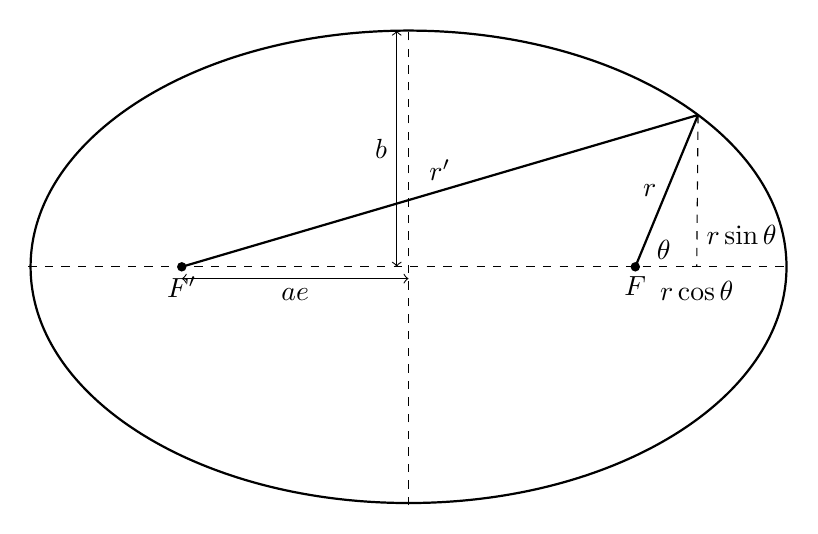
\begin{tikzpicture}[scale=3]

% Parameters
\def\a{1.6}
\def\b{1}
\def\e{0.6}
\def\c{\a*\e}

% Ellipse
\draw[thick] (0,0) ellipse ({\a} and {\b});

% Foci
\fill (-\c,0) circle (0.02) node[below] {$F'$};
\fill (\c,0) circle (0.02) node[below] {$F$};

% Axes
\draw[dashed] (-\a-.01,0) -- (\a+.01,0);
\draw[dashed] (0,-\b-.01) -- (0,\b+.01);

% Point on ellipse
\coordinate (P) at (40:{\a} and {\b});

% Radii
\draw[thick] (\c,0) -- (P) node[midway,left] {$r$};
\draw[thick] (-\c,0) -- (P) node[midway,above] {$r'$};

% Semi-major axis label
\draw[<->] (-\c,-0.05) -- (0,-0.05) node[midway,below] {$ae$};

% Semi-minor axis label
\draw[<->] (-0.05,0) -- (-0.05,\b) node[midway,left] {$b$};

% Angle theta
\node at ({\c+0.12},0.07) {$\theta$};

\draw[dashed] (P) -- (1.22, 0) node[right, yshift=.4cm] {$r\sin\theta$};

\node at (1.22, -.1) {$r\cos\theta$};

\end{tikzpicture}

Using the Pythagorean Theorem, we get that $$r'^2 = r^2 \sin^2\theta + (2ae + r \cos \theta)^2$$

Then, we get $$r'^2 = r^2 + 4ae(ae + r \cos\theta)$$, and substituting $r + r' = 2a$ and rearranging, we get that $$r = \frac{a(1-e^2)}{1+e\cos\theta}$$
\end{customproof}

\begin{exercise}
\

Prove that the total area of an ellipse is $$A = \pi ab$$
\end{exercise}

\begin{definition}[Conic Sections]
\

A conic section's eccentricity corresponds to the slope of the plane slicing the conic section. If $e = 1$, you get a \textbf{parabola}, given by $$r = \frac{2p}{1+\cos\theta}$$where $p$ is the singular focus of the parabola.

If $e > 1$, you get a hyperbola, given by $$r = \frac{a(e^2-1)}{1 + e\cos\theta}$$
\end{definition}

\begin{customproof}[Newton's Three Laws]
\

\begin{enumerate}
    \item An object at rest will stay at rest and an object in motion will stay in motion unless acted upon by an external force. $$p = mv$$
    \item The net force is equal to the object's mass times acceleration. $$F_\text{net} = ma$$
    \item For every action there is an equal and opposite reaction. 
\end{enumerate}
\end{customproof}

\begin{proposition}[Newton's Law of Universal Gravitation]
\

When one object's mass is much larger than the other, the orbit is roughly circular. Then, we can simplify Kepler's Third Law to read: $$P^2 = a^3 = kr^3$$with a constant $k$ to account for us using meters now. 

Now, note that $$P = \frac{2\pi r}{v}$$as the orbit's circumference divided by it's speed gives how long it takes to complete an orbit. Substituting, we get $$\frac{4\pi^2r^2}{v^2} = kr^3$$Rearranging and multiplying by $m$ yields $$m\frac{v^2}{r} = \frac{4\pi^2m}{kr^2}$$But the left side is centripetal force, so $$F_c = \frac{4\pi^2 m}{kr^2}$$

By Netwon's third law, $$F = \frac{4\pi^2M}{k' r^2}$$and letting $k'' = Mk = mk'$, we get $$F = \frac{4\pi^2 Mm}{k''r^2}$$ and again grouping constants we get $$F = G\frac{Mm}{r^2}$$
\end{proposition}

\begin{theorem}
\

Show that gravitational potential energy is given by $$U = -G \frac{mM}{r}$$
\end{theorem}

\begin{customproof}
\

By integrating force with respect to distance, we get $$U(r) = \int G\frac{mM}{r^2} = -G\frac{mM}{r}$$
\end{customproof}

\end{document}